\documentclass[12pt]{article}
\usepackage[utf8]{inputenc}
\usepackage[finnish]{babel}
\usepackage[T1]{fontenc}
\usepackage{setspace}
\usepackage{amsmath}
\usepackage{amssymb}
\usepackage{hyperref}
\usepackage{amsthm}
\usepackage{graphicx}
\theoremstyle{definition}
\newtheorem{maar}{Määritelmä}
\theoremstyle{plain}
\newtheorem{lause}{Lause}
\usepackage{csquotes}
\numberwithin{equation}{section}
\setlength{\parskip}{\medskipamount}
\setlength{\parindent}{0pt}
\setlength{\emergencystretch}{15pt}
\thispagestyle{empty}                   

\newcommand{\ee}[1]{e^{#1}}         

\newcommand{\viiva}{\mathop{\Bigg/}}
\newcommand{\sij}[3]{\viiva\limits_{\hspace*{-5mm}{#1}}^{\hspace*{5mm}{#2}}{#3}}

\title{Gammafunktio}
\author{Reetta Tervo}
\begin{document}
\maketitle

\newpage
\tableofcontents

\newpage
\section{Johdanto}
\onehalfspacing
Tämän tutkielman tavoitteena on esitellä gammafunktiota ja sen ominaisuuksia. Tutkielmassa olen keskittynyt tarkemmin gammafunktion ainutlaatuisuuteen ja siihen liittyviin ominaisuuksiin. Tämän lisäksi esittelen gammafunktion ja kertomafunktion välistä yhteyttä.

Gammafunktio on eräs kertomafunktion yleistyksistä, jota kuvataan symbolilla $\Gamma(x)$. Gammafunktio on erityinen, sillä se on kertomafunktion yleistyksistä ainoa, jonka logaritmi on konveksi eli se on \emph{logaritmisesti konveksi}. Tutkielmassa osoitan, että kaikki Bohr-Mollerupin -lauseen toteuttavat funktiot ovat yhteneviä gammafunktion kanssa.

Tutkielman alussa määrittelen gammafunktion ja kerron hieman sen taustasta. Tämän jälkeen seuraa Luku 3, \emph{Bohr-Mollerupin lause}, jossa käsittelen tarkemmin gammafunktiota. Bohr-Mollerupin -lauseen todistamisessa käytän apuna konveksisuuden, logaritmisen konveksisuuden ja gammafunktion määritelmiä. Gammafunktion todistamisessa käytän puolestaan apuna $\emph{Youngin}$ ja $\emph{Hölderin}$ epäyhtälöitä.

\newpage

\section{Gammafunktio}
Gammafunktion yleisin esitysmuoto on Leonard Eulerin vuonna 1729 määrittämä integraaliesitys
\begin{equation}\label{yhtalo:gammafunktio}
     \Gamma(x) = \int_{0}^{\infty} e^{-t} t^{x-1} dt,
\end{equation}
missä $\Gamma:(0,\infty)\rightarrow\mathbb{R}$ ja $x>0$.

\begin{center}
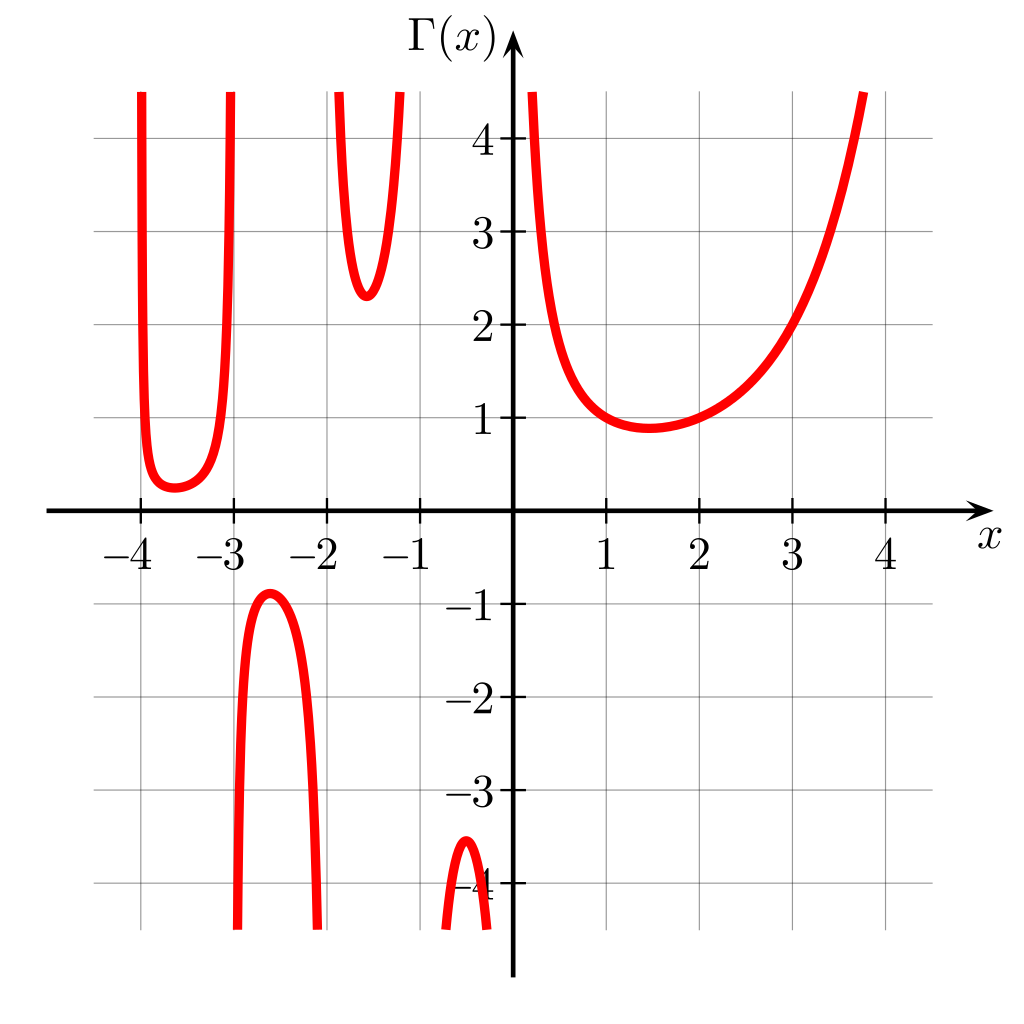
\includegraphics[width=0.7\textwidth]{Gamma-function.png} \newline
\caption{Gammafunktion kulkua välillä $[-4,4]$}
\end{center}
\newpage
Gammafunktio on epäoleellinen integraali. Tästä johtuen, tutkittaessa sen olemassaoloa, tulee se olla määriteltynä hyvin. Tällöin tutkitaan siis määrättyjä integraaleja
\begin{align*}
    (a) \int_{\epsilon}^{1} e^{-t} t^{x-1} dt \\
    (b) \int_{1}^{\delta} e^{-t} t^{x-1} dt.
\end{align*}

Tutkitaan ensin määrättyä integraalia $(a)$, kun $x>0$:\newline
Kun luku $t$ on positiivinen, niin integroitava osuus on pienempi kuin $t^{x-1}$. Näin saadaan
\begin{align*}
    e^{-t} t^{x-1} < t^{x-1}.
\end{align*} 
Tällöin voidaan arvioida integraalia ylöspäin seuraavasti 
\begin{align*}
    \int_{\epsilon}^{1} e^{-t} t^{x-1} dt < \int_{\epsilon}^{1} t^{x-1} dt = \Big/_\epsilon^1 {t^x}x^{-1} = {x}^{-1}-\epsilon^{x}{x}^{-1}.
\end{align*}
Kun $\epsilon \rightarrow 0$, niin $\epsilon^{x}x^{-1}\rightarrow 0$ ja tällöin myös $x^{-1}-\epsilon{^x}x^{-1} \rightarrow \frac{1}{x}$. Siispä, kun määrätyn integraalin $(a)$ alaraja lähestyy nollaa, niin epäoleellinen integraali on  rajoitettu välillä $(0, 1]$ ja raja-arvo
\begin{equation*}
    \lim_{\epsilon\to0}\int_{\epsilon}^{1}e^{-t}t^{x-1}dt
\end{equation*}
on olemassa. Täten voidaan todeta, että epäoleellinen integraali $\int_{0}^{1} e^{-t} t^{x-1} dt$ on olemassa ja se suppenee. \newline

Tutkitaan seuraavaksi määrättyä integraalia $(b)$, kun $x>0$: \newline
Kun luku $t$ on positiivinen, niin kaikki sarjan $e^t$ termit ovat positiivisia. Tällöin myös kaikilla kokonaisluvuilla $n$ pitää paikkaansa, että $e^t\ge\frac{t^n}{n!}$. Täten päästään epäyhtälöön $e^{-t}\le\frac{n!}{t^n}$ ja tästä edelleen $e^{-t}t^{x-1}\le{t^{-{n+1-x}}}{n!}$. Valitaan jokin $n>x+1$, jolloin saadaan epäoleelliselle integraalille yläraja $\delta=\frac{n!}{n-x}$. Tällöin
\begin{align*}
    \int_1^{\delta}e^{-t}t^{x-1}dt.
\end{align*}
Koska integraalin arvo kasvaa monotonisesti eli sen arvo kasvaa, kun $\delta$ kasvaa, niin raja-arvo 
\begin{align*}
    \lim_{\delta\to\infty}\int_1^{\delta}e^{-t}t^{x-1}dt
\end{align*}
on olemassa. Tällöin myös epäoleellinen integraali $\int_1^{\infty}e^{-t}t^{x-1}dt$ on olemassa.\newline

Nyt todettiin, että määrätyt integraalit $(a)$ ja $(b)$ ovat olemassa. Tällöin myös epäoleellinen integraali $(2.1)$ on olemassa, jolloin voidaan todetä, että gammafunktio on olemassa.



\subsection{Kertomafunktio}
\begin{maar}
(kertomafunktio)
Funktio $f: N \rightarrow N$ on kertomafunktio, jos seuraavat ehdot toteutuvat:
\begin{quote}
    $i)$ $f(1)=1$ \newline
    $ii)$ $f(n+1)=(n+1)f(n)$ \newline
    Kun ehdot $i)$ ja $ii)$ toteutuvat, niin voidaan merkitä $f(n)=n!$.
\end{quote}
\end{maar}
Kertomafunktio on monelle tuttu entuudestaan. Sille ominaista on arvojen erittäin nopea kasvu. Esimerkiksi luvun $4$ kertoma on $24$ ($4! = 1\cdot 2\cdot3\cdot4=24$), kun taas luvun $5$ kertoma on $120$ ($5! = 1\cdot2\cdot3\cdot4\cdot5=120$), joka on moninkertainen luvun $4$ kertomaan verrattuna.

Määritelmän 1, kohta $i)$ on selkeä, sillä luvun $1$ kertoma on luku itse eli $1!=1$. Kohta $ii)$ puolestaan on mielenkiintoinen, koska sen mukaan kertomafunktiolla on ominaisuus, että 
\begin{equation}
    (n+1)! = (n+1)n!.
\end{equation}
Koska gammafunktio on kertomafunktion yleistys, niin sille pätevät täysin samat ehdot kuin kertomafunktiolle. Gammafunktio siis toteuttaa kertomafunktion eli määritelmän 1 ehdot. Yhtälöstä $\eqref{yhtalo:gammafunktio}$ saadaan tutkittua ensimmäinen ehto laskemalla integraalin arvo muuttujan arvolla $1$. Tällöin
\begin{equation*}
    \Gamma(1)=\int_0^\infty e^{-t}t^{1-1}dt=\int_0^\infty e^{-t}t^{0}dt = \int_0^\infty e^{-t}dt = 1.
\end{equation*}
Toisen ehdon todistus tapahtuu \emph{Lause 3}:n todistuksen yhteydessä.
\begin{center}
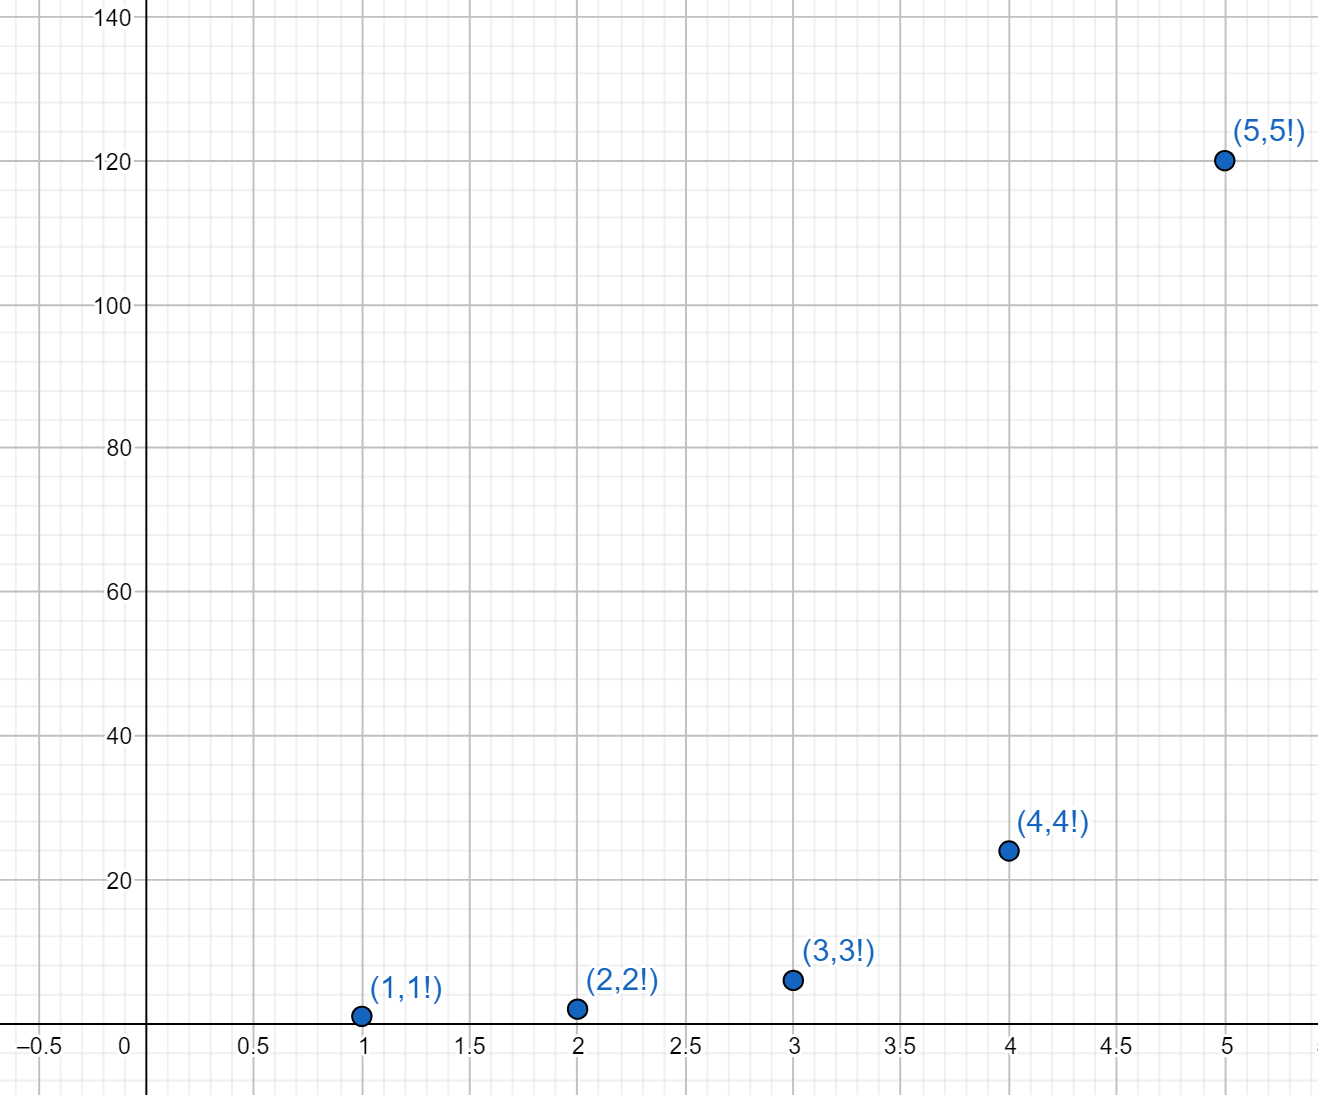
\includegraphics[width=0.8\textwidth]{kertomakuva.png} \newline
\caption{Kuvassa kertomafunktion arvoja pisteissä $(x,x!)$}
\end{center}

\newpage

\section{Bohr-Mollerupin lause}
\onehalfspacing
Bohr-Mollerupin lauseen mukaan gammafunktio on ainoa kertomafunktion yleistys, joka on logaritmisesti konveksi. Tämä ominaisuus tekee gammafunktiosta erityisen. Funktiota sanotaan konveksiseksi, kun sen kuvaaja on alaspäin kupera. Lauseen mukaan gammafunktion logaritmin kuvaaja on siis alaspäin kupera.
\newline

\begin{maar}
(konveksisuus) \label{maar: konveksisuus}
Olkoon $X\subset\mathbb{R}, t\in (0, 1)$ ja funktio \\ $f: X \rightarrow \mathbb{R}$. Funktio $f$ on \emph{konveksi}, jos kaikilla $x,y \in X$
\begin{equation}\label{yhtalo:konveksi}
    f(tx+(1-t)y) \le tf(x)+(1-t)f(y).
\end{equation}
\end{maar}


\begin{maar}
(logaritminen konveksisuus) \label{maar: logkonveksisuus}
Olkoon $X\subset\mathbb{R}, t \in (0, 1)$. Funktio $f: X \rightarrow \mathbb{R}$ on siis määritelty ja positiivinen. Funktio $f$ on \emph{logaritmisesti konveksi}, jos sen logaritmi on \emph{konveksi} eli $\log f(x)$ on konveksi.
\end{maar}

\begin{lause} \label{lause: young}
(Youngin epäyhtälö). Oletetaan, että $a$ ja $b$ ovat positiivisia reaalilukuja ja $q \in (0,1)$. Tällöin
\begin{equation}\label{yhtalo:youngi}
    a^{q}b^{1-q} \le qa+(1-q)b
\end{equation}
\end{lause}
\begin{proof}
Olkoon $a,b \ge 0$ ja $q \in (1,0)$. Kun luku jompi kumpi luvuista $a$ tai $b$ on nolla, niin epäyhtälö on tosi. Yhtäsuuruus pätee, jos ja vain jos $a=b$. Oletetaan, että $a,b > 0$. Käytetään apuna logaritmia ja tietoa siitä, että logaritmifunktio on konveksi.Tällöin saadaan
\begin{equation*}
    \log[a^{q}b^{1-q}] = \log[a^q] + \log[b^{1-q}] = q \log [a]+(1-q)\log [b] \le \log[qa+(1-q)b].
\end{equation*}
Yllä sovelletaan konveksisuuden määritelmän epäyhtälöä $\eqref{yhtalo:konveksi}$. Tämän lisäksi tiedetään, että logaritmifunktio on myös aidosti kasvava, jolloin saadaan haluttu tulos eli
\begin{equation*}
    a^{q}b^{1-q}\le qa+(1-q)b.
\end{equation*}
\end{proof}

\begin{lause} \label{lause: hölder}
(Hölderin epäyhtälö) Oletetaan, että $t \in (0,1)$. Tällöin 
\begin{equation}
    \int_{\mathbb{R}} |f(x)g(x)|dx \le \left( \int_{\mathbb{R}} |f(x)|^{\frac{1}{t}} \right)^{t}\left( \int_{\mathbb{R}} |g(x)|^{\frac{1}{1-t}}\right)^{1-t}.
\end{equation}
\end{lause}
\begin{proof}
Kun $\int_\mathbb{R}|f(x)|^{\frac{1}{t}}dx=0$,  niin $f(x)=0$. Tällöin pätee myös
\begin{equation}
    \int_{\mathbb{R}} |f(x)g(x)|dx=0.
\end{equation}
Vastaavasti myös $g(x)=0$, kun $\int_{\mathbb{R}}|g(x)|^{\frac{1}{1-t}}dx=0$. Koska lause pätee näillä arvoilla, voidaan olettaa nämä integraalit positiivisiksi.

Olkoon $t\in(0,1).$ Käytetään nyt \emph{Youngin epäyhtälöä}, \eqref{yhtalo:youngi}, lauseen todistuksessa, jolloin saadaan
\begin{equation*}
    \frac{|f(x)||g(x)|}{\left(\int_{\mathbb{R}}|f(x)|^{\frac{1}{t}}\right)^{t}\left(\int_{\mathbb{R}}|g(x)|^{\frac{1}{1-t}}\right)^{1-t}} \le t\frac{|f(x)|^{\frac{1}{t}}}{\left(\int_{\mathbb{R}}|f(x)|^{\frac{1}{t}}df\right)^{t}}+(1-t)\frac{|g(x)|^{\frac{1}{1-t}}}{\left(\int_{\mathbb{R}}|g(x)|^{\frac{1}{1-t}}dx\right)^{1-t}}.
\end{equation*}
Integroidaan epäyhtälöä puolittain, yli reaaliakselin, jolloin saadaan
\begin{equation*}
     \frac{|f(x)||g(x)|}{\left(\int_{\mathbb{R}}|f(x)|^{\frac{1}{t}}\right)^{t}\left(\int_{\mathbb{R}}|g(x)|^{\frac{1}{1-t}}\right)^{1-t}}\le t+1-t=1.
\end{equation*}
Näin päästään haluttuun muotoon, joka oli
\begin{equation*}
    \int_{\mathbb{R}} |f(x)||g(x)|dx \le \left( \int_{\mathbb{R}} |f(x)|^{\frac{1}{t}} \right)^{t}\left( \int_{\mathbb{R}} |g(x)|^{\frac{1}{1-t}}\right)^{1-t}.
\end{equation*}

\end{proof}

\begin{lause}
(gammafunktio) Gammafunktio  toteuttaa seuraavat ehdot:
\begin{quote}
    i) $\Gamma(1)=1$ \newline
    ii) $\Gamma(x+1)=x\Gamma(x)$ \newline
    iii) $\Gamma(x)$ on logaritmisesti konveksi.
\end{quote}
\end{lause}

\begin{proof}
Ehto $i)$ saadaan suoraan sijoittamalla luku $1$ yhtälöön \eqref{yhtalo:gammafunktio}, kun $x>0$:
\begin{align*}
    \Gamma(1) = \int_0^\infty e^{-t}t^{1-1} dt = \int_0^\infty e^{-t}dt = 1.
\end{align*}
Ehto $ii)$ puolestaan voidaan osoittaa todeksi, kun sijoitetaan yhtälöön \eqref{yhtalo:gammafunktio} $x$:n paikalle $x+1$, kun $x>0$
\begin{equation}\label{yhtalo:joku}
    \Gamma(x+1)=e^{-t}t^{(x+1)-1} = e^{-t}t^{x}.
\end{equation}
Nyt osittaisintegroidaan integraali \eqref{yhtalo:joku}
\begin{align*}
    \Gamma(x+1) & = \int_{\epsilon}^{\delta} e^{-t} t^{x} dt \\
    & = \Big/_\epsilon^\delta -e^{-t}t^{x}+x\int_\epsilon^\delta e^{-t}t^{x-1}dt \\
    & = e^{-\epsilon}\epsilon^{x}-e^{-\delta}\delta^{x}+x\int_\epsilon^\delta e^{-t}t^{x-1}dt.
\end{align*}

Kun $\epsilon\rightarrow0$, niin $\epsilon^x\rightarrow0$ ja tällöin myös $e^{-\epsilon}\epsilon^x \rightarrow0$. Näin osittaisintegraalin tuloksen ensimmäinen termi katoaa. Lisäksi tiedetään, että $e^{-\delta}\delta^{x} < \frac{n!}{\delta^{n-x}}$. Nyt, kun $\delta\rightarrow\infty$, niin luku $\frac{n!}{\delta^{n-x}}\rightarrow0.$ Tällöin myös $e^{-\delta}\delta{^x}\rightarrow0$ ja osittaisintegroinnin tuloksen toinenkin termi katoaa. Kun kaksi ensimmäistä termiä katoavat, niin jäljelle jää 
\begin{align*}
   \Gamma(x+1)=x\int_\epsilon^\delta e^{-t}t^{x-1}dt.
\end{align*}

Siis $\Gamma(x+1) = x\Gamma(x)$ eli ehto $ii)$ on myös tosi.

Kolmas todistus on huomattavasti haastavampi. Ehdon $iii)$ mukaan gammafunktion, $\Gamma(x)$, tulee olla logaritmisesti konveksi eli funktion $\log\Gamma(x)$ tulee olla konveksi.

Käytetään kolmannen ehdon todistuksessa apuna \emph{Hölderin epäyhtälöä}. Merkitään $g(x) = \log\Gamma(x)$. Funktion $g(x)$ tulee olla \emph{koveksi}, jotta kolmas ehto toteutuu.\newline
Olkoon $x,y\in(0,\infty)$ ja $z\in(0,1)$. Sijoitetaan gammafunktion yhtälöön \eqref{yhtalo:gammafunktio} muuttujan paikalle arvo $zx+(1-z)y$ seuraavasti
\begin{equation*}
    \Gamma(zx+(1-z)y)=\int_{0}^{\infty}e^{-t}t^{zx+(1-z)y-1}dt = \int_{0}^{\infty}(e^{-t}t^{x-1})^{z}(e^{-t}t^{x-1})^{1-z}dt.
\end{equation*}
Nyt yhtälö on muodossa, johon voidaan soveltaa Hölderin epäyhtälöä. Näin saadaan
\begin{equation*}
    \Gamma(zx+(1-z)y)\le \left( \int_{0}^{\infty}(e^{-t}t^{x-1})^{z}dt\right)^{z}\left(\int_{0}^{\infty}(e^{-t}t^{x-1})^{1-z}dt \right)^{z}=\Gamma(x)^{z}\Gamma(y)^{1-z}.
\end{equation*}
Nyt otetaan logaritmi puolittain ja käytetään logaritmin summaussääntöä hyväksi, jolloin päästään logaritmisen konveksisuuden ehtoon eli
\begin{equation*}
    \log\Gamma(zx+(1-z)y)\le z\log\Gamma(x)+(1-z)\log\Gamma(y).
\end{equation*}
Näin saatiin todistettua kolmas ehto, eli gammafunktio toteuttaa kaikki lauseen ehdot. \newline
\end{proof}

\begin{lause}
(Bohr-Mollerupin lause)
\newline
Jos funktio $f(x)$ toteuttaa seuraavat kolme ehtoa, niin se on gammafunktio:
\begin{quote}
i) $f(1)=1$ \newline
ii) $f(x+1)=xf(x)$ \newline
iii) Funktio $f(x)$ on logaritmisesti konveksi funktio.
\end{quote}
\end{lause}

\begin{proof}
Aikaisemmin todettiin, että gammafunktio toteuttaa nämä kolme ehtoa. Voidaan siis olettaa, että on olemassa ainakin yksi funktio, joka toteuttaa edellä mainitut ehdot ja  Bohr-Mollerupin lauseen mukaan gammafunktio on ainoa tällainen funktio. Täytyy siis osoittaa, että funktio, joka toteuttaa nämä ehdot, on yhtenevä gammafunktion kanssa.

Valitaan funktio $f$ ja oletetaan, että se toteuttaa nämä kolme ehtoa. Ensimmäisen ja toisen ehdon seurauksena riittää, että tarkastellaan vain tilannetta, jossa $x\in (0,1)$. Lisäksi soveltamalla logaritmin summaussääntöä ehtoon $ii)$ seuraa
\begin{equation} \label{yhtalo:logfx}
    \log [f(x+1)]=\log[xf(x)]=\log [f(x)]+\log[x].
\end{equation}
Koska funktio $f$ on oletuksen mukaan logaritmisesti konveksi, on sen logaritmi tällöin kasvava. Valitaan luku $n\in\mathbb{N}$ sekä välit $[n,n+1]$ ja $[n+1,n+1+x]$, joiden päätepisteiden erotusosamäärät noudattavat seuraavaa epäyhtälöä
\begin{equation*}
    \frac{\log f(n+1)-\log f(n)}{n+1-n}\le\frac{\log f(n+1+x)-\log f(n+1)}{n+1+x-(n+1)}.
\end{equation*}
Avaamalla sulkeet ja käyttämällä logaritmin laskusääntöjä, saadaan epäyhtälö seuraavaan muotoon
\begin{equation*}
    \log \frac{f(n+1)}{f(n)} \le \frac{\log f(n+1+x)-\log f(n+1)}{x}.
\end{equation*}
Kohdasta $ii)$ seuraa, että funktio $f(n+1)$ on luvun $n$ kertoma. Tällöin 
\begin{equation} \label{yhtalo:logan}
    \log n \le \frac{\log f(n+1+x)-\log n!}{x}.
\end{equation}
Koska $x\in(0,1)$, voidaan muodostaa epäyhtälö myös välien $[n+1,n+1+x]$ ja $[n+1, n+2]$ päätepisteiden erotusosamäärille vastaavalla tavalla. Tällöin
\begin{equation*}
    \frac{\log f(n+1+x)-\log f(n+1)}{n+1+x-(n+1)}\le\frac{\log f(n+2)-\log f(n+1)}{n+2-(n+1)}.
\end{equation*}
Sievennetään saatua epäyhtälöä, yhdistetään se yhtälöön \eqref{yhtalo:logan} ja kerrotaan molemmat puolet luvulla $x$. Näin saadaan
\begin{equation} \label{yhtalo:epayhtalo}
    x\log n \le \log f(n+1+x) -\log n! \le x\log (n+1).
\end{equation}
Nyt sovelletaan yhtälöä \eqref{yhtalo:logfx} toistuvasti tulokseen seuraavasti:
\begin{align*}
    \log f(n+1+x) & = \log f(x+n) + \log (x+n) \\
    & = \log f(x+n-1) + \log [(x+n)(x+n-1)] \\
    & = \log f(x+n-2)+\log [(x+n)(x+n-1)(x+n-2)] \\
    & \dots \\
    & = \log f(x) + \log [(x+n)(x+n-1)\dots(x+1)x].
\end{align*}
Näin saatiin tulos $\log f(n+1+x) = \log f(x) + \log [(x+n)(x+n-1)\dots(x+1)x]$. Nyt sijoitetaan se epäyhtälöpariin \eqref{yhtalo:epayhtalo} ja vähennetään kummaltakin puolelta $x\log n$, jolloin vasemmalle puolelle jää vain luku $0$ seuraavasti
\begin{equation*}
    0 \le \log f(x) -\log \left[ \frac{n^xn!}{x(x+1)\cdots(x+n)}\right] = x\log \left(1+\frac{1}{n}\right).
\end{equation*}
Kun $n\rightarrow\infty$, niin $\log (1+\frac{1}{n})\rightarrow \log (1)$. Koska $\log (1)=0$, lähestyy oikean puoleinen termi nollaa eli $x\log (1+\frac{1}{n})\rightarrow 0$. Tästä päästään yksikäsitteisesti muotoon  $\log f(x) = \log \left[\frac{n^xn!}{x(x+1)\cdots(x+n)}\right]$. Näin ollen, kun $n$ kasvaa rajatta, niin
\begin{equation*}
    f(x)=\lim_{n\to\infty} \frac{n^xn!}{x(x+1)\cdots(x+n)}.
\end{equation*}
Funktio $f(x)$ siis toteuttaa kaikki kolme ehtoa. Tämän lisäksi tiedämme, että myös gammafunktio, $\Gamma(x)$, toteuttaa ne. Kuitenkin juuri johdettu muoto pitää paikkaansa myös tilanteessa, jossa funktion $f(x)$ tilalle vaihdetaan funktio $\Gamma(x)$. Siispä funktio $f(x)$ on yhtenevä gammafunktion kanssa. Näin saadaan
\begin{equation*}
    \Gamma(x) = \lim_{n\to\infty}\frac{n^xn!}{x(x+1)\cdots(x+n)}.
\end{equation*}

\end{proof}

\newpage
\doublespacing
\section{Kirjallisuutta}
[1] Artin, Emil \emph{The Gamma Function}, Holt, Rineheart and Winston, 1964, kääntänyt englanniksi Bulter, Michael

[2] \url{http://en.citizendium.org/wiki/Gamma_function}, Viitattu 19.4.2019

[3] Makkonen, Lauri \emph{Gammafunktio}, Pro gradu -tutkielma,\\ Helsingin yliopisto, 2018. \url{http://hdl.handle.net/10138/230938}

[4] \emph{GeoGebra}, versio GeoGebra 6.0.533.0-wgraphing (08 April 2019)

[5] \url{https://upload.wikimedia.org/wikipedia/commons/thumb/3/3e/Gamma-function.svg/1024px-Gamma-function.svg.png}, Viitattu 19.4.2019

[6] \url{http://functions.wolfram.com/GammaBetaErf/Gamma/introductions/Gammas/01/}, Viitattu 19.4.2019

[7] \url{http://mathworld.wolfram.com/GammaFunction.html}, Viitattu 19.4.2019


\end{document}